\documentclass[tikz,border=10pt]{standalone}
\usetikzlibrary{arrows.meta, positioning, calc, decorations.pathreplacing}
\usepackage{amsmath}
\usepackage{amssymb}

\begin{document}
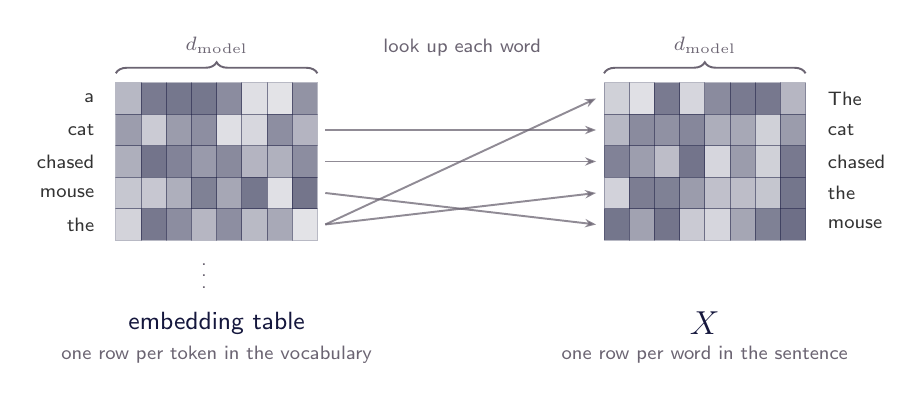
\begin{tikzpicture}[
    every node/.style={font=\sffamily},
]

\definecolor{c1}{HTML}{15173D}   % the input: embeddings and X
\definecolor{c2}{HTML}{982598}
\definecolor{c3}{HTML}{E491C9}
\definecolor{c4}{HTML}{F1E9E9}
\definecolor{axiscolor}{HTML}{333333}
\definecolor{labelcolor}{HTML}{6B6472}

\def\cw{0.32}   % cell width
\def\ch{0.40}   % row height

% ================================================================
%   embedding table  top-left (0, 5.6)     6 rows shown x 8 cols
%   X                top-left (6.2, 5.6)   5 rows x 8 cols
%   rows of the table are tokens, rows of X are positions in the sentence
% ================================================================

% ---------------------------------------------------------------- the table
\foreach \tok/\r in {a/0, cat/1, chased/2, mouse/3, the/4} {
    \node[font=\sffamily\scriptsize, text=axiscolor, anchor=east]
        at (-0.15, 5.6-\r*\ch-0.5*\ch) {\tok};
    \foreach \c in {0,...,7} {
        \pgfmathsetmacro{\op}{0.12 + 0.5*rnd}
        \fill[c1, opacity=\op] (\c*\cw, 5.6-\r*\ch-\ch) rectangle ++(\cw, \ch);
        \draw[c1, opacity=0.3, line width=0.3pt]
            (\c*\cw, 5.6-\r*\ch-\ch) rectangle ++(\cw, \ch);
    }
}
\node[font=\sffamily\scriptsize, text=labelcolor, anchor=east] at (1.28, 3.25)
    {$\vdots$};

\draw[decorate, decoration={brace, amplitude=4pt}, labelcolor, line width=0.7pt]
    (0, 5.72) -- (2.56, 5.72);
\node[font=\sffamily\scriptsize, text=labelcolor, anchor=south] at (1.28, 5.85)
    {$d_{\mathrm{model}}$};

\node[font=\sffamily\small, text=c1] at (1.28, 2.55) {embedding table};
\node[font=\sffamily\scriptsize, text=labelcolor] at (1.28, 2.15)
    {one row per token in the vocabulary};

% ---------------------------------------------------------------- X
\foreach \tok/\r in {The/0, cat/1, chased/2, the/3, mouse/4} {
    \foreach \c in {0,...,7} {
        \pgfmathsetmacro{\op}{0.12 + 0.5*rnd}
        \fill[c1, opacity=\op] (6.2+\c*\cw, 5.6-\r*\ch-\ch) rectangle ++(\cw, \ch);
        \draw[c1, opacity=0.3, line width=0.3pt]
            (6.2+\c*\cw, 5.6-\r*\ch-\ch) rectangle ++(\cw, \ch);
    }
    \node[font=\sffamily\scriptsize, text=axiscolor, anchor=west]
        at (8.92, 5.6-\r*\ch-0.5*\ch) {\tok};
}

\draw[decorate, decoration={brace, amplitude=4pt}, labelcolor, line width=0.7pt]
    (6.2, 5.72) -- (8.76, 5.72);
\node[font=\sffamily\scriptsize, text=labelcolor, anchor=south] at (7.48, 5.85)
    {$d_{\mathrm{model}}$};

\node[font=\sffamily\large, text=c1] at (7.48, 2.55) {$X$};
\node[font=\sffamily\scriptsize, text=labelcolor] at (7.48, 2.15)
    {one row per word in the sentence};

% ---------------------------------------------------------------- lookups
\foreach \from/\to in {4/0, 1/1, 2/2, 4/3, 3/4} {
    \draw[-{Stealth[length=4pt]}, line width=0.7pt, labelcolor, opacity=0.75]
        (2.66, 5.6-\from*\ch-0.5*\ch) -- (6.1, 5.6-\to*\ch-0.5*\ch);
}
\node[font=\sffamily\scriptsize, text=labelcolor] at (4.4, 6.05) {look up each word};

\end{tikzpicture}
\end{document}
